\chapter{Implementation}\label{implementation}

The most promising vector tile specification was proposed by Mapbox.
\marginpar{The Mapbox Vector Tile Specification is compared with other vector tile formats in chapter \ref{vector-tile-formats}}
They provide many open source tools to manage vector tiles. We tried not to implement tools which already exists and instead use as many existing tools as possible. Because of this our implementation consists mostly of docker containers which do a specific task.

\section{Data Sources}
\label{data-sources}

Making a map involves finding the right data slice in the right
data sources.

\subsection{OpenStreetMap}

The biggest part of our data originates from published OpenStreetMap snapshots. The OpenStreetMap data is used to provide the detailed parts of the map and is the cornerstone of the entire map.

We import selected key value pairs and their geometries of the entire OpenStreetMap database from Planet OSM \footnote{\url{http://planet.osm.org/}}.


\subsection{Curated OpenStreetMap Data}

Certain OpenStreetMap data like borders and land polygons are very sensitive for change.
The OpenStreetMapData\footnote{\url{http://openstreetmapdata.com/}}
project takes care of alot of issues that happen with coastlines
and provide it in a convenient format.

We use the following data from OpenStreetMapData:

\begin{itemize}
\item Water polygons
\end{itemize}

\section{Natural Earth}

The Natural Earth \footnote{\url{http://www.naturalearthdata.com/}} dataset provides manually curated data of cultural and physical features of the world. Natural earth data is especially useful at higher levels when it matters alot what to display when.

We use the following data from Natural Earth:

\begin{itemize}
\item Rankings of big cities
\item Major lakes
\item Country and administrative borders
\end{itemize}

\section{Classification}
\label{classification}

The OpenStreetMap tagging schema has developed into a complex taxonomy of real-world feature classes and objects. \cite[p. 15]{haklay2008openstreetmap}. Map designers don't want to design
for each distinct object specifically which is why Mapbox and others abstract distinct key value pairs into so called feature classes.

Mapbox calls those feature class simply class.

Mapping created key value pairs into categories cannot be automated
and there is no standard. This is why we have done it by hand.

A map designer that wants to style agricultural areas does not care
what type of field it is.

\begin{table}[]
\centering
\caption{My caption}
\label{my-label}
\begin{tabular}{llll}
Key      & Value      & Class       & Type           \\
landuse  & farm       & agriculture & orchard        \\
building & farm       & agriculture & farm           \\
landuse  & farmland   & agriculture & farmland       \\
landuse  & farmyard   & agriculture & farmyard       \\
landuse  & allotments & agriculture & allotments     \\
landuse  & vineyard   & agriculture & vineyard       \\
landuse  & vineyard   & agriculture & plant\_nursery
\end{tabular}
\end{table}

\subsection{Classification Format}

We created the classifications in a YAML based format.
Where each key in \texttt{classifications} denotes the classification name. The elements within each classification (e.g. \texttt{driveway} or \texttt{main} are the class name and the values below the class name (e.g. \texttt{primary}, \texttt{primary\_link} the OSM values to match. We do not explicitly match the OSM keys as well - only the values.

\begin{yamlcode}
classifications:
  road:
    highway:
    - motorway
    - motorway_link
    - driveway
    main:
    - primary
    - primary_link
    - trunk
    - trunk_link
    - secondary
    - secondary_link
    - tertiary
    - tertiary_link
\end{yamlcode}

\subsection{Code Generation}

We take the readable classification format and generate immutable SQL
functions we can use in our queries.
The example above will result in the following function.

\begin{sqlcode}
CREATE OR REPLACE FUNCTION classify_road(type VARCHAR)
RETURNS VARCHAR AS $$
  BEGIN
    RETURN CASE
      WHEN type IN ('motorway','motorway_link','driveway') THEN 'highway'
      WHEN type IN ('primary','primary_link',
                    'trunk','trunk_link',
                    'secondary','secondary_link',
                    'tertiary','tertiary_link') THEN 'main'
    END;
  END;
$$ LANGUAGE plpgsql IMMUTABLE;
\end{sqlcode}

\subsection{Use in Vector Tile Generation}

Classifications are then baked into vector tile attributes
of geometries.

\begin{sqlcode}
SELECT
  geometry,
  classify_road(type) AS class,
  type AS type
FROM osm_roads
\end{sqlcode}

\section{Relative Importance}
\label{localrank}

To reduce label density on lower zoom levels but still contain all data in e.g. zoom level 14 the \texttt{localrank} attribute indiciates how
important a label is compared to the labels in its neighbourhood.

\subsection{Calculating Rank}

And then create the local rank for each tile in a 128 px grid when returning the POIs.

In the best case scenario one would create a function that
ranks each individual point of interest. In this case we only ranked the most important features.

\subsubsection{Order Features by their Types}

\begin{sqlcode}
CREATE OR REPLACE FUNCTION localrank_poi(type VARCHAR) RETURNS INTEGER
AS $$
BEGIN
  RETURN CASE
    WHEN type IN ('station', 'subway_entrance', 'park',
                  'cemetery', 'bank', 'supermarket', 'car',
                  'library', 'university', 'college', 'police',
                  'townhall', 'courthouse') THEN 2
    WHEN type IN ('nature_reserve', 'garden', 'public_building') THEN 3
    WHEN type IN ('stadium') THEN 90
    WHEN type IN ('hospital') THEN 100
    WHEN type IN ('zoo') THEN 200
    WHEN type IN ('university', 'school', 'college', 'kindergarten') THEN 300
    WHEN type IN ('supermarket', 'department_store') THEN 400
    WHEN type IN ('nature_reserve', 'swimming_area') THEN 500
    WHEN type IN ('attraction') THEN 600
    ELSE 1000
  END;
END;
$$ LANGUAGE plpgsql IMMUTABLE;
\end{sqlcode}


\subsubsection{Calculate Rank of Features}

The rank is calculated across a grid of 128 pixels. Our most
important features from the \texttt{localrank\_poi} function will
also be the most relevant POIs.

\begin{sqlcode}
SELECT
  geometry,
  rank() OVER (PARTITION BY LabelGrid(geometry, 128 * !pixel_width!)
               ORDER BY localrank_poi(type) ASC) AS localrank,
FROM osm_poi
\end{sqlcode}

\section{Data Style}

The data style is a description of all the feature classes such as landuse, water or roads. This description was invented by Mapbox.

The format of a data style looks like this:

\begin{yamlcode}
_prefs: 
  disabled: []
  inspector: false
  mapid: ''
  rev: ''
  saveCenter: true
attribution: ''
center: 
  - 21.7969
  - 34.6694
  - 3
description: Open Streets
Layer: 
    # All layer definitions come here
maxzoom: 14
minzoom: 0
name: Open Streets
\end{yamlcode}

\section{Layer Definition}\label{layer_definition}
A layer definition describes a view on the data. It can consist of multiple data sources. In the figure below the layer is a view and the definition of this view is a graphic definition.

\begin{figure}[h]
  \centering
  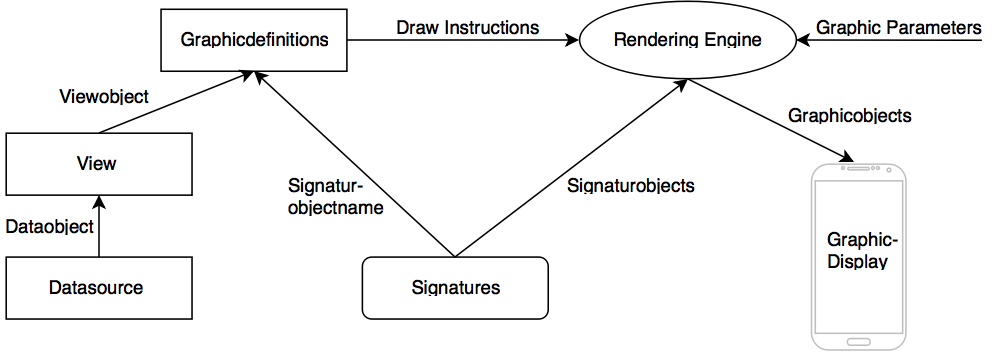
\includegraphics[width=1\textwidth]{images/graphic_definition.png}
  \caption{General graphic definition}
\end{figure}

A layer definition looks like this:
\begin{yamlcode}
- id: landuse
Datasource:
    extent: -20037508.34,-20037508.34,20037508.34,20037508.34
    host: db
    port: 5432
    user: osm
    password: osm
    dbname: osm
    key_field: osm_id
    table: |-
        (
            SELECT osm_id, class, type, geometry
            FROM osm_landusages
            WHERE geometry && !bbox!
            AND z(!scale_denominator!) > 5
        
        ) as data
    type: postgis
fields:
    osm_id: Number
    class: String
    type: String
properties:
    "buffer-size": 4
\end{yamlcode}


\subsection{Buffers}\label{buffers}
The buffer value on a layer defines how many pixels around each tile will be included. It is necessary to ensure correct rendering across tile boundaries. This value is individual for each layer and depends on the type of data. Buffers for layers containing labels should have a large buffers size such as 128 pixels, whereas a layer like landuse does only need a buffers size of 4 pixels. In general, the buffer size should be set to the minimum to keep the size of the vector tiles as low as possible.\footnote{\url{https://www.mapbox.com/help/source-manual/#buffers}}

\begin{figure}[h]
  \centering
  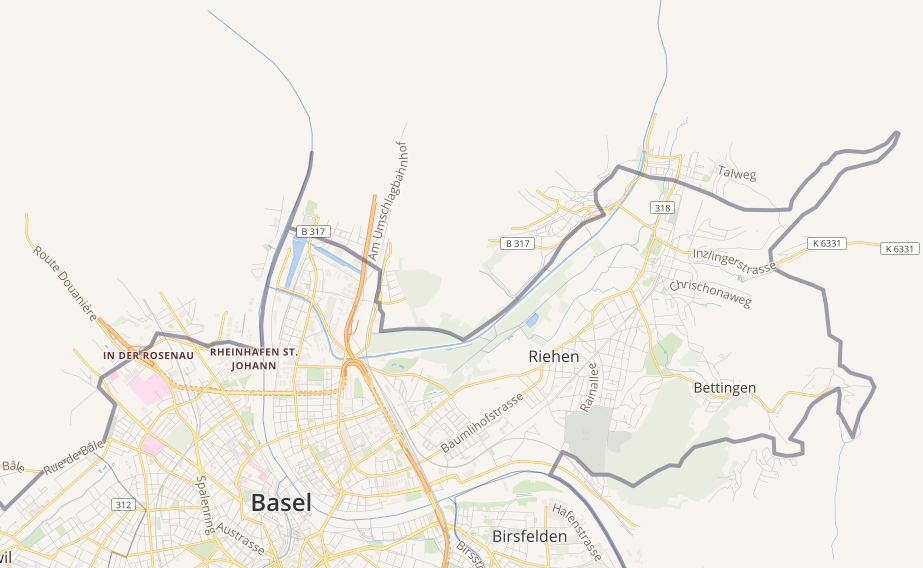
\includegraphics[width=1\textwidth]{images/buffer.png}
  \caption{Example for buffer values}
\end{figure}

The figure above is a good example to see the result of a buffer value. We can see that there are rivers but no other data, therefore the rivers must have a larger buffer value that the other layers.

\subsubsection{Overzooming}\label{overzooming}
The min- and maxzoom values define on which zoom levels there is data. This does not mean that it is not possible to zoom deeper in that the maxzoom value.
Overzooming defines to term of displaying data at higher zoom levels.\footnote{\url{https://www.mapbox.com/help/source-manual/#overzooming}}
This allows us to show data on higher zoom levels, without generating vector tiles for these zoom levels.
Mapbox has defined a rule of thumb for vector tiles. Vector tiles are useful for about 4-6 levels of overzooming. If I have a vector tile on zoom level 10, it can be stretched out up to zoom level 14 or 16.  



\subsection{Zoomlevel Reference}\label{zoomlevel_reference}

% Please add the following required packages to your document preamble:
% \usepackage{graphicx}
\begin{table}[H]
\centering
\resizebox{\textwidth}{!}{%
\begin{tabular}{l|ccccccccccccccc}
 & \multicolumn{1}{l}{z0} & \multicolumn{1}{l}{z1} & \multicolumn{1}{l}{z2} & \multicolumn{1}{l}{z3} & \multicolumn{1}{l}{z4} & \multicolumn{1}{l}{z5} & \multicolumn{1}{l}{z6} & \multicolumn{1}{l}{z7} & \multicolumn{1}{l}{z8} & \multicolumn{1}{l}{z9} & \multicolumn{1}{l}{z10} & \multicolumn{1}{l}{z11} & \multicolumn{1}{l}{z12} & \multicolumn{1}{l}{z13} & \multicolumn{1}{l}{z14} \\ \hline
landuse &  &  &  &  &  & x & x & x & x & x & x & x & x & x & x \\
waterway &  &  &  &  &  &  &  &  & x & x & x & x & x & x & x \\
water & x & x & x & x & x & x & x & x & x & x & x & x & x & x & x \\
aeroway &  &  &  &  &  &  &  &  &  &  &  &  & x & x & x \\
barrier\_line &  &  &  &  &  &  &  &  &  &  &  &  &  &  & x \\
building &  &  &  &  &  &  &  &  &  &  &  &  &  & x & x \\
landuse\_overlay &  &  &  &  &  &  &  & x & x & x & x & x & x & x & x \\
tunnel &  &  &  &  &  &  &  &  &  &  &  & x & x & x & x \\
road &  &  &  &  &  & x & x & x & x & x & x & x & x & x & x \\
bridge &  &  &  &  &  &  &  &  &  &  &  &  & x & x & x \\
admin & x & x & x & x & x & x & x & x & x & x & x & x & x & x & x \\
country\_label &  & x & x & x & x & x & x & x & x & x & x & x & x & x & x \\
marine\_label &  & x & x & x & x & x & x & x & x & x & x & x & x & x & x \\
state\_label &  &  &  &  & x & x & x & x & x & x & x & x & x & x & x \\
place\_label &  &  &  &  & x & x & x & x & x & x & x & x & x & x & x \\
water\_label &  &  &  &  &  &  &  &  &  &  & x & x & x & x & x \\
poi\_label &  &  &  &  &  &  &  &  &  &  &  &  &  &  & x \\
road\_label &  &  &  &  &  &  &  &  & x & x & x & x & x & x & x \\
waterway\_label &  &  &  &  &  &  &  &  & x & x & x & x & x & x & x \\
housenum\_label &  &  &  &  &  &  &  &  &  &  &  &  &  &  & x
\end{tabular}
}
\caption{Shows which feature set is included on which zoom level}
\label{my-label}
\end{table}
